\documentclass[twoside]{../zirkelblatt1415}
\usepackage{mathtools}
\usepackage{wrapfig}
\usepackage{tabto}
\usepackage{booktabs}
\usepackage{relsize}
\let\raggedsection\centering

\theoremstyle{definition}
\newtheorem{defn}{Definition}[section]
\newtheorem{defn'}{Vorläufge Definition}[section]
\newtheorem{axiom}[defn]{Axiom}
\newtheorem{bsp}[defn]{Beispiel}

\theoremstyle{plain}

\newtheorem{prop}[defn]{Proposition}
\newtheorem{motto}[defn]{Motto}
\newtheorem{wunder}[defn]{Wunder}
\newtheorem{ueberlegung}[defn]{Überlegung}
\newtheorem{lemma}[defn]{Lemma}
\newtheorem{kor}[defn]{Korollar}
\newtheorem{hilfsaussage}[defn]{Hilfsaussage}
\newtheorem{satz}[defn]{Satz}
\newtheorem{thm}[defn]{Theorem}

\theoremstyle{remark}
\newtheorem{bem}[defn]{Bemerkung}
\newtheorem{warnung}[defn]{Warnung}
\newtheorem{aufg}[defn]{Aufgabe}

\definecolor{darkred}{rgb}{0.7,0,0}
\definecolor{shadecolor}{rgb}{.95,.95,.95}

\newcommand{\defeq}{\vcentcolon=}

\DeclareMathOperator{\ld}{ld}
\newcommand{\RR}{\mathbb{R}}
\newcommand{\CC}{\mathbb{C}}

\usepackage[T1]{fontenc}
\usepackage{libertine}

\begin{document}

\maketitleCustom{Klassen 10/11/12}{\textbf{\textsf{%
  Der Residuensatz \\
  \normalsize Zirkelzettel vom 20. März 2015}}}

\begin{center}
%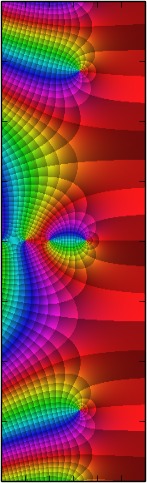
\includegraphics[angle=90]{zeta-function-complex}

\vspace{0.4cm}
\begin{minipage}{0.9\textwidth}
\scriptsize Die Werte der Riemannschen~$\zeta$-Funktion auf einem Streifen um den
Ursprung in der komplexen Zahlen\-ebene (um 90~Grad gedreht).
\url{http://en.wikipedia.org/wiki/File:Riemann-Zeta-Detail.png}\par
\end{minipage}
\end{center}

\vspace{1em}
{\renewcommand{\addvspace}[1]{\vskip0.6em}
\tableofcontents%
}


\section{Das komplexe Kurvenintegral}

In der Schule integriert man Funktionen~$f : \RR \to \RR$ längs Intervallen,
also gewissen Ausschnitten der reellen Zahlengerade. Man schreibt dafür
\[ \int_a^b f(x) \,dx \qquad\text{oder}\qquad \int\limits_{[a,b]} f(x) \,dx. \]
Wir möchten nun Funktionen~$f : \CC \to \CC$ längs \emph{Kurven in der
komplexen Zahlenebene} integrieren. Die Werte solcher Funktionen sind also
komplexe Zahlen, die von einem komplexen (statt reellen) Parameter abhängen.
Ist~$L$ eine solche Kurve, so schreiben wir \[ \int_L f(z) \,dz \] für das
Integral von~$f$ längs~$L$. Im Spezialfall, dass~$L$ \emph{geschlossen ist}
(also Anfangs- und Endpunkt von~$L$ übereinstimmen), so schreiben wir zur
Betonung gelegentlich \[ \oint_L f(z) \,dz. \]

Wie berechnet man ein solches Integral? Wie ist ein solches Integral überhaupt
definiert? Dafür verwendet man \emph{Parametrisierungen}. Eine Parametrisierung
einer Kurve~$L$ ist eine bijektive Abbildung~$\gamma : [a,b] \to \CC$, deren
Werte genau die Punkte von~$L$ ablaufen. Hat man eine solche Parametrisierung
gefunden, so definiert man
\[ \int_L f(z) \,dz \defeq \int_a^b f(\gamma(t)) \, \gamma'(t) \,dt. \]

\begin{bem}Ein und dieselbe Kurve~$L$ kann durch mehrere verschiedene
Abbildungen parametrisiert werden. Man kann zeigen, dass der Wert des
Kurvenintegrals aber bei jeder Parametrisierung der gleiche ist.\end{bem}

\begin{bem}Für die Ableitung~$\gamma'$ einer komplexwertigen Funktion~$\gamma$
gelten dieselben Rechenregeln wie für die aus der Schule bekannten
reellwertigen Funktionen. Zum Beispiel ist die Ableitung der Funktion~$\gamma$
mit~$\gamma(t) = 7t + i t^2$ die Funktion~$\gamma'$ mit~$\gamma'(t) = 7 + 2ti$.
Die Zahl~$i$ wird also einfach als Konstante betrachtet.
\end{bem}

\begin{aufgabe}{Beispiele für Parametrisierungen}
Welche Kurven werden durch die folgenden Abbildungen parametrisiert?
\begin{enumerate}
\item $\gamma : [0,1] \to \CC,\ t \mapsto 3+t.$
\item $\gamma : [0,2] \to \CC,\ t \mapsto t + i t^2.$
\item $\gamma : [0,2\pi] \to \CC,\ t \mapsto e^{it}.$
\end{enumerate}
\emph{Tipp für Teilaufgabe~c):} Es gilt~$e^{it} = \cos(t) + i \sin(t)$. Wo
liegt diese Zahl in der komplexen Zahlenebene?
\end{aufgabe}

\begin{aufgabe}{Parametrisierungen von Kreisen}
Finde eine Parametrisierung des \ldots
\begin{enumerate}
\item Einheitskreises,
\item um den Faktor~$r$ vergrößerten Einheitskreises,
\item Kreises mit Radius~$r$ und Mittelpunkt~$p$.
\end{enumerate}
\fixlistspacing
\end{aufgabe}

\begin{aufgabe}{Die Mutter aller komplexen Kurvenintegrale}
Berechne das Integral von~$1/z$ längs des Einheitskreises.
\end{aufgabe}

\begin{aufgabe}{Weitere wichtige komplexe Kurvenintegrale}
Der Integrationsweg~$L$ sei in den folgenden Fällen stets der Einheitskreis.
\begin{enumerate}
\item Was ist~$\int_L z \,dz$?
\item Was ist~$\int_L z^2 \,dz$?
\item Was ist~$\int_L \frac{1}{z^2} \,dz$?
\end{enumerate}
\end{aufgabe}

\begin{aufgabe}{Vergleich mit dem gewöhnlichen Integral}
Sei~$[a,b]$ ein Intervall auf der reellen Zahlengerade. Dieses können wir auch
als (ungekrümmte) Kurve~$L$ in der komplexen Zahlenebene auffassen. Was ist der
Zusammenhang zwischen dem altbekannten Integral~$\int_a^b$ und dem
Kurvenintegral~$\int_L$? Beweise deine Vermutung, indem du eine
Parametrisierung von~$L$ angibst und die Definition des Kurvenintegrals
verwendest!
\end{aufgabe}


\section{Die Laurentwicklung von komplexen Funktionen}

Eine \emph{Laurentreihe} mit Entwicklungspunkt~$c$ ist eine Reihe der Form
\[ \cdots + a_{-2} (z-c)^{-2} + a_{-1} (z-c)^{-1} + a_0 + a_1 (z-c) + a_2 (z-c)^2 + \cdots, \]
wobei die Koeffizienten~$a_n$ beliebige komplexe Zahlen sein können. Eine
Laurentreihe mit Entwicklungspunkt~$0$ ist also von der Form
\[ \cdots + a_{-2} z^{-2} + a_{-1} z^{-1} + a_0 + a_1 z + a_2 z^2 + \cdots. \]
Viele komplexe Funktionen lassen sich auf diese Form bringen.

\begin{bsp}Die Laurentreihe des Polynoms~$5 z^2 - 3z + 8$ mit
Entwicklungspunkt~$0$ lässt sich sofort ablesen: Die meisten Koeffizienten sind
Null. Die einzigen Ausnahmen sind~$a_0 = 8$, $a_1 = -3$ und~$a_2 = 5$.\end{bsp}

\begin{aufgabe}{Beispiele für Laurententwicklungen}
Finde jeweils eine Laurententwicklung mit Entwicklungspunkt~$0$ von \ldots
\begin{enumerate}
\item $\frac{1}{1 - z}$,
\item $\frac{1}{1 - z^2}$,
\item $e^{\frac{1}{z}}$,
\item $\frac{1}{(z - i) (z + i)}$.
\end{enumerate}
\emph{Tipp:} Verwende die Formel für die geometrische Reihe, $\sum_{n=0}^\infty
q^n = \frac{1}{1 - q}$. Für Teilaufgabe~c) ist die Identität~$e^z = 1 + z + z^2/2 +
z^3/3! + z^4/4! + \cdots$ nützlich.
\end{aufgabe}

Der Koeffizient~$a_{-1}$ ist besonders wichtig. Er heißt auch \emph{Residuum}
der Laurentreihe an dem gegebenen Entwicklungspunkt. Für die Integration längs
eines beliebig kleinen Kreises~$K$ um den Ursprung gilt nämlich
\[ \int_K (\cdots + a_{-1} z^{-1} + \cdots) \,dz = 2\pi i \cdot a_{-1}. \]
All die anderen Koeffizienten spielen also keine Rolle!

\begin{aufgabe}{Baby-Version des Residuensatzes}
Beweise diese Formel.
\end{aufgabe}


\section{Der Residuensatz}

% Wegunabhängigkeit
% holomorphe und meromorphe Funktionen

\end{document}
